%%%%%%%%%%%%%%%%%%%%%%%%%%%%%%%%%%%%%%%%%%%%%%%%%%%%%%%%%%%%%%%%%%%%%%
%%
%% RStemplate.tex
%%
%%   このテンプレートは,LaTeX-2e 専用です。
%%
%%  
%%
%%%%%%%%%%%%%%%%%%%%%%%%%%%%%%%%%%%%%%%%%%%%%%%%%%%%%%%%%%%%%%%%%%%%%%
\documentclass[a4jsme]{jsmepaper}
\usepackage{rsympo}
\usepackage{jtygm}
\usepackage{bm}
\usepackage{epic,eepic}
% \usepackage[dvips]{graphicx}
\usepackage[dvipdfmx]{graphicx}
\usepackage{amsmath}


%2024追記 奈良
\def\acknowledgements{\par
  {\centering{\bfseries 謝\hskip1zw 辞}\hskip1zw \par}
\ignorespaces}
\def\endacknowledgements{\par}
\newcommand\figref[1]{図~\ref{fig:#1}}
\newcommand\tabref[1]{表~\ref{tab:#1}}


\pagestyle{empty}
%---------------------------------------------------------------------
% 和文主題
%---------------------------------------------------------------------
\title{
 Phase Odometry:Wi-Wi搬送波位相とオドメトリを\\相補的に考慮したグラフ最適化によって累積誤差を解消する\\移動ロボットの軌跡推定
}  
%---------------------------------------------------------------------
% 和文副題
%---------------------------------------------------------------------
\subtitle{
}
%---------------------------------------------------------------------
% 英文主題
%---------------------------------------------------------------------
\etitle{
 Phase Odometry: Trajectory Estimation for Mobile Robots via Graph Optimization to Mitigate Error Accumulation by \\ Complementing Wi-Wi Carrier Wave Phases and Odometry
}
%---------------------------------------------------------------------
% 英文副題
%---------------------------------------------------------------------
\esubtitle{
}
%---------------------------------------------------------------------
% 著者和文名
%---------------------------------------------------------------------
\jauthor{
    奈良 貴明$^{*1}$,\ \
    岡田 佳都$^{*1}$,\ \
    小島 匠太郎$^{*1}$,\ \
    横田 将輝$^{*1}$,\ \
    Ranulfo Bezerra$^{*1}$,\ \\
    大野 和則$^{*1}$,\ \
    志賀 信泰$^{*2}$,\ \
    安田 哲$^{*2}$,\ \ 
    滝沢 賢一$^{*2}$,\ \
    田所 諭$^{*1}$
}
%---------------------------------------------------------------------
% 著者英文名
%---------------------------------------------------------------------
\eauthor{
    Takaaki NARA$^{*1}$,\ \
    Yoshito OKADA$^{*1}$,\ \
    Shotaro KOJIMA$^{*1}$,\ \
    Yoshiki YOKOTA$^{*1}$,\ \
    Ranulfo Bezerra$^{*1}$,\ \ 
    Kazunori OHNO$^{*1}$,\ \
    Nobuyasu SHIGA$^{*2}$,\ \
    Satoshi YASUDA$^{*2}$,\ \ 
    Kenichi TAKIZAWA$^{*2}$,\ \
    Satoshi TADOKORO$^{*1}$
}
%---------------------------------------------------------------------
% 著者の所属の和文
%---------------------------------------------------------------------
\jaffiliation{
  $^{*1}$ & 東北大学情報科学研究科(〒980-8579 宮城県仙台市青葉区荒巻字青葉6-3-09)nara.takaaki@rm.is.tohoku.ac.jp\\
  $^{*2}$ & 情報通信研究機構(〒184-8795 東京都小金井市貫井北町4-2-1)
}
%---------------------------------------------------------------------
% 著者の所属の英文
%---------------------------------------------------------------------
\eaffiliation{
  $^{*1}$ Graduate School of Information Sciences, Tohoku University, \\
  6-3-09 Aramaki Aza Aoba, Aoba-ku, Sendai-shi, Miyagi 980-8579, Japan \\
  $^{*2}$ National Institute of Information and Communications Technology, \\
  4-2-1, NukuiKitamachi, Koganei-shi, Tokyo 184-8795, Japan
}
%---------------------------------------------------------------------
% 英文の概要
%---------------------------------------------------------------------
\abstract{%
We propose a localization method for mobile robots based on the radio wave phase measurements from multiple wireless fixed bases. 
In the proposed method, we define a graph where the fixed bases and the robot positions at each time step are represented as nodes, and the measured movements between these nodes as edges. 
Since phase measurements have high accuracy but contain a 2$\pi$ ambiguity, we introduce edges based on the phase differences between measurements and edges based on the robot's wheel odometry, which are less accurate but free from ambiguity. 
We estimate the positions of both the robot and the fixed bases by solving an unconstrained nonlinear least-squares problem, which minimizes the error between the predicted and measured edge values. 
In this presentation, we report the results of simulation and real-world experiments on the estimation accuracy of the proposed method.
}
%---------------------------------------------------------------------
% キーワード
%---------------------------------------------------------------------
\keywords{Localization, Mobile robot, Wireless two-way interferometry(Wi-Wi)}
%---------------------------------------------------------------------
\begin{document}
\maketitle
\thispagestyle{empty}
%
\section{緒言}
%(研究分野の紹介) 
電波の搬送波位相を用いた位置推定技術は,電波強度に基づく距離計測や符号を用いた擬似距離計測などと比較して,高い計測精度を持つことから自動運転分野などで注目されている\cite{gnss_autonomou_vehicles}.
搬送波位相計測による代表的な位置推定手法としては,RTK-GNSS(Real Time Kinematic Global Navigation Satellite System)\cite{RTK-GNSS}がある.
RTK-GNSSを用いることで,数センチの精度で受信アンテナの位置を推定でき,ドローン\cite{RTK-M300},農業分野\cite{RTK-Agriculture},建設分野\cite{six-dump}など様々な分野で活用されている.
一方で,GNSSを使用するには衛星が直視できる環境が必要であることや,大気や地磁気等の自然現象の影響によって精度が低下する問題\cite{gnss_error,STANKOV2007485}が存在する.

\begin{figure}[tb]
    \centering
    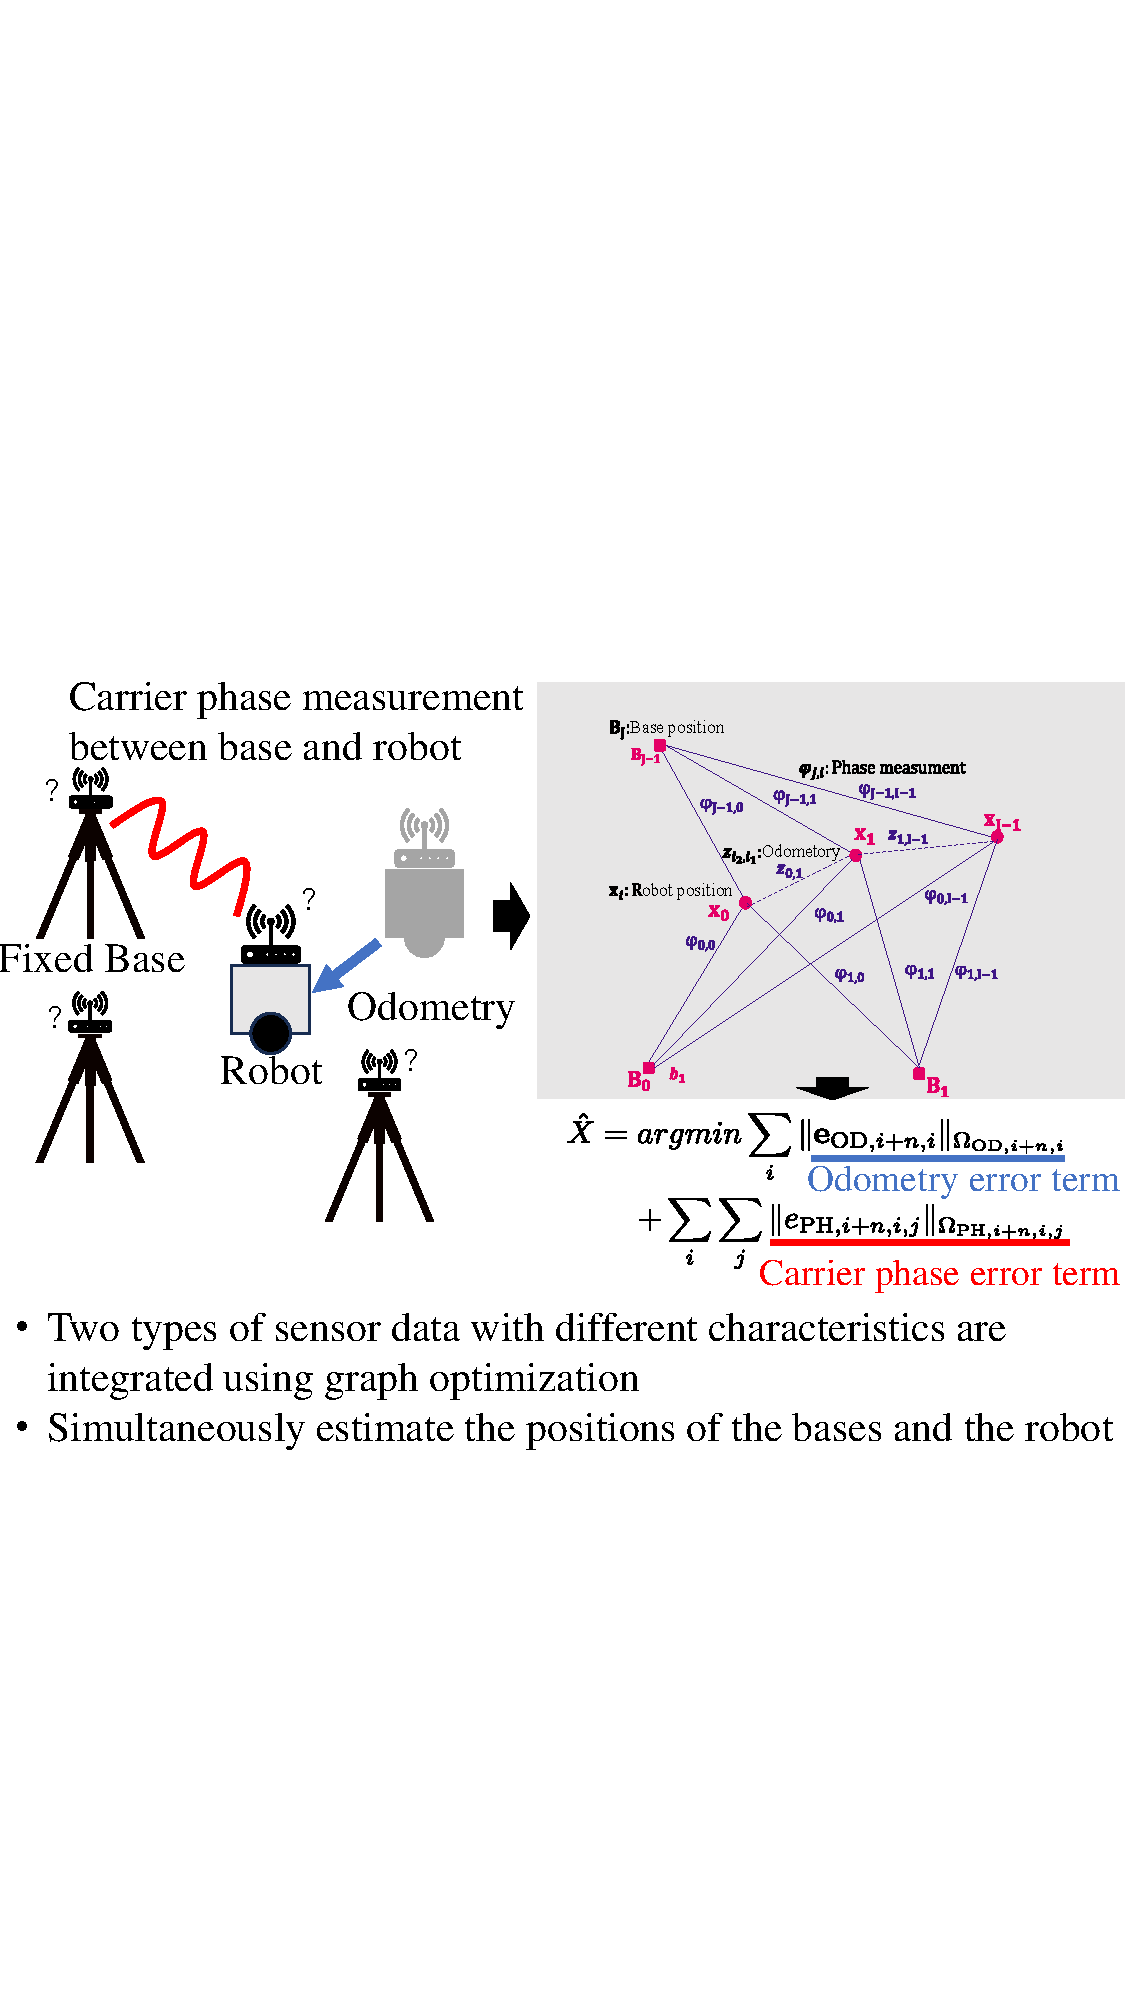
\includegraphics[width=0.99\linewidth]{figures/Fig1.pdf}
    \caption{The simultaneous estimation of the robot's position and the fixed bases' position is based on graph optimization using carrier phase and odometry measurements.}
    \label{fig:fig1}
\end{figure}

%(背景) 
著者らはRTK-GNSSとは別のアプローチとして,無線を用いた高精度な時刻同期技術である「無線双方向時刻同期技術」(Wireless two-way interferometry:Wi-Wi)\cite{Shiga2017,Yasuda2019}に基づく搬送波位相計測による位置推定手法を研究している.
搬送波位相計測では,無線端末の内部時計のズレが距離計測に反映される問題がある.この問題を解決するには,GNSSのように高精度だが非常に高価な原子時計を用いるか,接続範囲に制限がある有線接続によって高精度な時刻同期を行う必要がある.
そのため,これまでの技術では,移動ロボットで手軽に搬送波位相計測を利用することは困難であった.
それに対して,Wi-Wiは双方向の無線通信プロトコルによって通信デバイスの時刻を民生品レベルの無線通信によってサブナノ秒レベルで同期できる技術である.
我々は,\figref{fig1}に示すように,Wi-Wi端末をロボットと環境両方に設置し,Wi-Wiによる高精度時刻同期に基づいて計測される高精度な位相情報用いることで,既存の技術よりも高い精度を持つ位置推定手法の実現を目指している.

%(課題)
しかし,Wi-Wiによる位置推定を実現するうえで課題が2つある.
1つ目は,搬送波位相計測に存在する$2\pi$の不定性である.
不定性とは,位相計測値が$2\pi$周期で繰り返し計測されることである.
位相計測値はアンテナ間の距離に応じて変化するが,不定性があるため,直接アンテナ間の絶対距離を計測することは難しい.
そのため,位相計測値を直接利用するだけでは,正確な位置推定が困難であり,位相計測値の処理に工夫が必要である.
2つ目は,ユーザが固定局を自由に設置する問題設定である.
設置した固定局の位置関係が正確には分からない状態から,不定性の伴う位相計測値に基づいて固定局の位置関係や移動ロボットの位置を導出する必要がある.

%(解決方法) 
本研究では,これらの課題を解決するために,計測時刻の異なる搬送波位相の差分と,タイヤの回転量などから算出できるオドメトリを組み合わせた,グラフ最適化による位置推定手法を提案する.
%(提案手法の特徴)
提案手法の特徴は,計測精度が高い反面,不定性を持つ搬送波位相に基づくエッジと,精度は劣るが不定性のない車輪の回転量などから得られるロボットの移動量に基づくエッジを,位置推定に用いるグラフ構造に導入する.
それによって各計測値に累積した誤差を相補的に抑制する.
また,環境中に配置する固定局も未知パラメータとして扱うことで,固定局配置に関する事前情報が乏しい場合においても,ロボットが環境中を移動するだけで,固定局の位置も含めてロボットの軌跡を推定できる.

%(本論文での貢献)
本論文では,シミュレーションを用いて提案手法の特性を解析するとともに,屋内環境での実機実験を行い提案手法の推定精度を検証した.
実験の結果,電波による位置推定が難しい屋内環境において移動ロボットの位置を1m以下の精度で推定し,固定局の位置では最小で0.11mの精度で推定できることを確認した.

\section{関連研究}
%Wi-Wiの話
無線双方向時刻同期技術(Wi-Wi:Wireless two-way interferometry)では,無線端末が双方向に搬送波位相を計測し,時刻のズレを補正することで,端末間の高精度時刻同期を実現する.
本研究で用いるWi-Wi端末は920MHz帯の搬送波を用いる小型通信端末として実装されており,30ナノ秒の時刻同期精度と20ピコ秒の位相同期(ジッター)精度を実現している\cite{ouchi2024evaluation}.
Wi-Wiを利用した研究には,高精度な時刻同期機能を用いた無線ネットワークの遅延制限に関する研究\cite{Yamasaki2021}がある.
また,大気中での伝搬特性の変化を利用して大気中の水蒸気量の推定を行う研究\cite{Yasuda2019}も存在する.
しかし,ロボットなどの移動体の位置推定にWi-Wiを用いた研究は,著者らの先行研究\cite{rsj2021_nara,rsj2022_nara,ziku2023_nara}以外にはまだない.
そこで,本研究では,移動ロボットと環境中にWi-Wi端末を設置し,環境中の固定局と移動ロボットのWi-Wi端末間での搬送波位相計測を用いたグラフ最適化ベースの位置推定手法を提案する.

%グラフSLAMの話
グラフベースの最適化手法は,ロボットの軌跡推定において,移動量や位置の誤差を最小化するための強力なアプローチであり,特にカメラ,LiDAR(Light Detection And Ranging),オドメトリを用いたSLAM(Simultaneous Localization and Mapping)技術が盛んに研究されている\cite{grisetti2010tutorial,graph_slam_urban_mapping,graph_slam_2012}.

%それをもとにグラフと搬送波を組み合わせた方法
搬送波を用いた高精度な位置推定手法としては,計測時刻の違うGNSS搬送波位相の差分を用いるTDCP(Time differenced carrier phase)を活用した手法が研究されている\cite{TDCP2008,TDCP2022}.
搬送波位相の時刻差分を用いることで,搬送波の不定性を排除し,マルチパス環境下での高精度な推定結果が報告されている.
また,TDCPとグラフベースの最適化を組み合わせた手法として,単一のGNSS受信機のみで高精度な軌跡推定を行うGNSS Odometryが提案されている\cite{suzuki2022gnss}.
上記のGNSS搬送波を用いた手法では,人工衛星からの搬送波が良好に受信できる環境では優れた位置推定精度を提供するが,信号が遮蔽される屋内環境での利用は難しい.
一方,提案手法では,GNSSが利用できないような環境でも無線固定局を配置することで,固定局の位置とロボットの軌跡を同時に推定できる手法を目指す.

\newpage

\section{オドメトリと搬送波位相差分を組合せた\\グラフ最適化による軌跡推定}
\subsection{概要}
提案手法では,環境中に設置した複数のWi-Wi端末を固定局とし,移動ロボットにはロボットの移動量が計測可能なオドメトリセンサおよび,固定局と通信可能なWi-Wi端末が搭載されている.
固定局は複数台存在し,その位置関係は未知として扱う.
搬送波位相計測値は,通信可能な固定局すべてから計測でき,どの固定局からの通信なのか識別可能である.
移動ロボットは,環境中を移動中にオドメトリの計測と搬送波位相の計測を行う.
一般的にオドメトリ計測のほうが更新周期が速いため,本手法では,搬送波位相計測を行ったタイミングでの位置をオドメトリ計測値とし,オドメトリと搬送波位相の計測タイミングは同期されているものとする.

\subsection{グラフ構造と記号の定義}
最適化するグラフ構造を\figref{graph_structure}に示す.
グラフには,J個の固定局ノード($\mathbf{B_j}$)とI個のロボットノード($\mathbf{x}_i$)が存在する.
$i$はロボットが搬送波位相計測を行った位置である.
ロボットノード間にはオドメトリ計測値$\mathbf{z}$に基づくエッジが存在する.
ロボットノードと固定局ノード間には搬送波位相計測値$\phi$に基づくエッジが存在する.

まず,提案手法における状態変数の集合は以下に定義される.
\begin{figure}[tb]
    \centering
    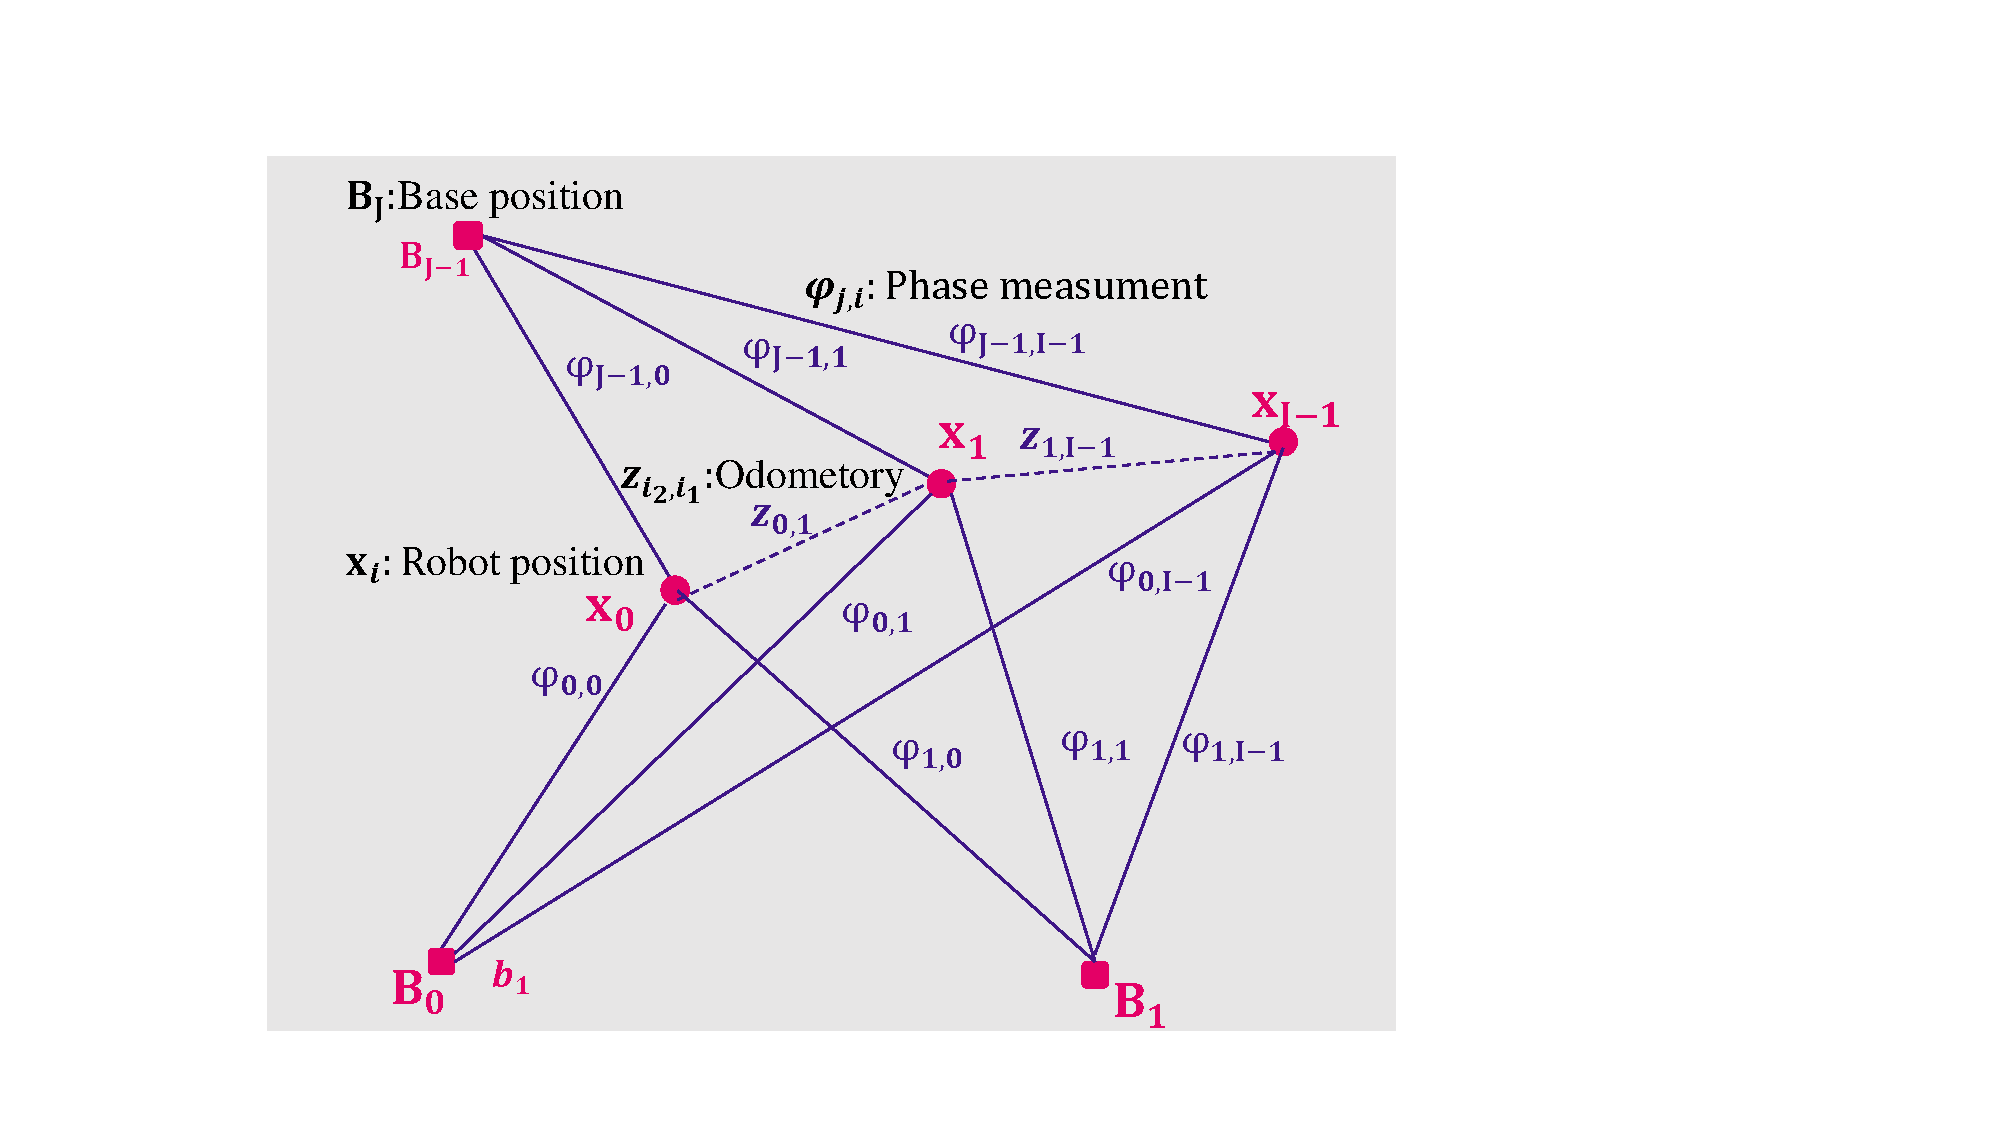
\includegraphics[width=0.95\linewidth]{figures/graph.pdf}
    \caption{Graph structure to be optimized in the proposed method.}
    \label{fig:graph_structure}
\end{figure}
$\mathbf{H}$はロボットのオドメトリ座標系から推定座標系への座標変換行列である.

\begin{equation}
    \mathbf{X} = \left[\mathbf{\hat{x}}_0 \ \mathbf{\hat{x}}_1 \  \mathbf{\hat{x}}_2 \ \cdots \mathbf{\hat{x}}_{I-1} \  \mathbf{\hat{B}}_0 \ \mathbf{\hat{B}}_1 \ \cdots \mathbf{\hat{B}}_{J-1} \  \mathbf{\hat{H}} \right]
\end{equation}
各ノードでの状態変数は以下で定義される
\begin{equation}
   \mathbf{\hat{x}}_i = \left[\mathbf{p}_i \ \theta_{i}\right]
\end{equation}
\begin{equation}
   \mathbf{\hat{B}}_j = \left[\mathbf{p'}_j\right]
\end{equation}
ここで,$\mathbf{p}$は2次元推定座標系での各ノードの位置(x,y)を表す.$\theta_{i}$はX-Y平面内での回転角を表す.
固定局は等方性を持ったアンテナを想定しているため回転角の情報は含まれない.

グラフ最適化によるポーズ推定問題では,すべてのノードに対して並進,及び回転の操作を実施しても,グラフ内のコスト関数は変化しないため,推定解が一意に定まらないケージ自由度と呼ばれる問題がある.
そこで,2次元空間における推定では,$\mathbf{B_0}$を原点とし,原点から見て$\mathbf{B_1}$方向をx軸とする.
すなわち,$\mathbf{B}_0$は(0,0),$\mathbf{B}_1$は(0,$p'_{y,1}$)として最適化が行われる.

\subsection{目的関数の定式化}
最適化によって最小化する目的関数はオドメトリ計測に基づく誤差関数$\mathbf{e}_{\mathrm{OD}}$と位相計測に基づく誤差関数$e_{\mathrm{PH}}$と対角成分に各計測値に関する重みを持つ情報行列$\Omega$を用いて定義される.

% なお,4価では,n=1として$i$番目のオドメトリ計測値とその次のオドメトリ計測値間を評価する.
\begin{align}
    \hat{X} = argmin\sum_{i}\|\mathbf{e}_{\mathrm{OD},i+n,i}\|_{\Omega_{\mathrm{OD},i+n,i}} \\
    +\sum_{i}\sum_{j}\|e_{\mathrm{PH},i+n,i,j}\|_{\Omega_{\mathrm{PH},i+n,i,j}}
\end{align}

\subsection{オドメトリによる誤差関数}
本節では,オドメトリ計測による誤差関数の定義を行う.
提案手法では一般的なグラフSLAM\cite{graph_slam}で用いられるオドメトリ計測による誤差関数を用いる.
ロボットのオドメトリ座標系での状態は以下に定義される.
\begin{equation}
    \mathbf{x}_i = [\mathbf{p}_i \ \theta_i]
\end{equation}
$i$番目の状態$\mathbf{x}_i$と$i$から$n$後の状態$\mathbf{x}_{i+n}$間のオドメトリ計測値$\mathbf{z}_{i+n,i}$は各ロボット固有の計測モデル関数$\mathbf{h}$と計測ノイズ$\mathbf{w}_{i+n,i}$を用いて以下で定義される.
\begin{equation}
    \mathbf{z}_{i+n,i} = \mathbf{h}(\mathbf{x}_{i+n},\mathbf{x}_{i})+\mathbf{w}_{i+n,i}
\end{equation}

$i$番目の状態の推定値$\mathbf{\hat{x}}_i$と$i$から$n$後の状態の推定値$\mathbf{\hat{x}}_{i+n}$間での誤差関数はオドメトリ計測値$\mathbf{z}_{i+n,i}$用いて以下で定義される.
\begin{equation}
    \mathbf{e}_{\mathrm{OD},i+n,i} = \left(\mathbf{\hat{x}}_{i+n}-\mathbf{\hat{x}}_{i}\right)-\mathbf{\hat{H}}\mathbf{z}_{i+n,i}
\end{equation}
\begin{equation}
    \|\mathbf{e}_{\mathrm{OD},i+n,i}\|_{\Omega_{\mathrm{OD}}} = \mathbf{e}_{\mathrm{OD},i+n,i}{\Omega}_{\mathrm{OD},i+n,i}\mathbf{e}_{\mathrm{OD},i+n,i}
\end{equation}

\subsection{搬送波位相による誤差関数}
Wi-Wiから得られる搬送波の位相計測値は,アンテナ間を搬送波が伝搬する間の位相変化量$\phi_D$と,計測開始時からの$\phi_D$の変化量を半波長分位相が回転するごとに計測値をアンラップする整数バイアス$K_i$および計測ノイズ$w^\phi_{i,j}$を用いて以下で定義される\cite{Peng2017}.
\begin{equation}
     \phi_{i,j}=\phi_{D,i,j}+\frac{1}{2}{\pi}K_i+w^\phi_{i,j}
\end{equation}
Wi-Wiは計測開始時からの搬送波位相変化量をアンラップすることで位相計測の不定性に対応している.しかし,この手法では,反射波のなどの影響を受けた際に整数バイアスが間違って処理されてしまい,その後の計測値に誤差が累積していく問題がある.
そのため,提案手法では,$i$番目の計測位置でのロボットノードと固定局ノード間で誤差関数を定義するのではなく,$i$番目の計測位置と$i+n$番目の計測位置での位相計測値の差分を計測することで,累積した誤差の影響を抑制する.
2つのロボットノード間で計測された位相に計測誤差がなければ,その差分はロボットノードと固定局ノード間の絶対距離の差分と等しくなることを用いて不定性と累積誤差の影響を考慮した誤差関数を定義する.ここで,$\lambda$は搬送波の波長を表し,位相値にかけることで距離の変化量となる.
\begin{equation}
    e_{\mathrm{PH},i+n,i,j} = \left(|\mathbf{\hat{p}}_{i+n}-\mathbf{\hat{B_j}}|-|\mathbf{\hat{p}}_{i}-\mathbf{\hat{B}_j|}\right)-\lambda(\phi_{i+n,j}-\phi_{i,j})
\end{equation}
\begin{equation}    
    \|e_{\mathrm{PH},i+n,i,j}\|_{\Omega_{\mathrm{PH},i+n,i,j}} = e_{\mathrm{PH},i+n,i,j}\Omega_{\mathrm{PH},i+n,i,j}e_{\mathrm{PH},i+n,i,j}
\end{equation}

\section{シミュレーションによる提案手法の評価実験}
オドメトリに基づく誤差関数と搬送波位相計測に基づく誤差関数を組み合わせた効果をシミュレーション環境において評価した.
比較条件として,オドメトリ情報のみ,位相情報のみ,それらを組合せた提案手法を比較する.
シミュレーション環境はROS 1(Noetic)上に構築した.
提案手法は,非線形最適化ソルバーであるCeres Solver\cite{ceres-solver}を用いてROSノードとして実装した.
実験に使用したPCとソルバの諸元を\tabref{simpc}に示す.

\input{tables/simpc}

\subsection{実験条件}
シミュレーションは屋内空間におけるX-Y平面上での運用を想定し,10m$\times$10mの空間における2次元の位置推定問題を取り扱う.
つまり,高さ方向の推定は行わず,固定局とロボットに搭載されたWi-Wi端末は同じ高さにあると想定する.
空間の四隅に固定局を4台配置する.
ロボットは$(x,y)=(1,1)$mの地点からスタートし,空間を周回しながら空間の中心$(5,5)$mへ移動する.
各固定局との位相計測とオドメトリ計測は20Hzで行われる.
位相計測値には平均0m,標準偏差0.01mの正規分布に則るノイズを加えた.
オドメトリ計測値には1mの移動量あたり,平均0m,標準偏差0.1mの正規分布に則るノイズを並進方向に,平均0rad,標準偏差0.1radのノイズを回転成分に加えた.
推定は,新たな計測データを取得するたびに最適化計算を行うオンライン推定として行った.

比較条件は,オドメトリのみ,位相情報のみ,提案手法の3条件で比較を行う.
固定局の位置は位相情報のみと,提案手法で推定される.
固定局の初期値として最適化に用いた値を\tabref{initial}に示す.
固定局の真値からそれぞれ1m程度ずれた位置を設定した.
オドメトリのみは条件では,最適化を用いた位置推定は行われず計測値をそのまま用いる.
位相情報のみと提案手法では,最適化を用いた位置推定が行われる.
位相情報のみの推定では,ロボットノードの初期値は,前回の推定結果を初期値として用いた.
提案手法の推定では,オドメトリの計測値をロボットノードの初期値として用いた.


\subsection{実験結果}
\figref{trajectory_sim}(a),(b),(c)に各条件で推定されたロボットの軌跡と推定された固定局の位置を示す.
\figref{trajectory_sim}(d)に各条件でのロボットの軌跡推定誤差をユークリッド距離で計算し,横軸をロボットの移動距離でプロットしたものを示す.
オドメトリのみの軌跡では,徐々に計測誤差が累積していることが確認できる.
位相のみの推定では,経路上に推定結果がプロットされているが,時折経路から外れた推定結果が見られる.
提案手法では,座標(9,9)mの曲がりかど付近から推定結果が経路上に収束し,その後は,0.1m程度の誤差で軌跡を推定できている.

\figref{trajectory_sim}(e)に固定局$\mathbf{B}_2$に関する推定誤差を同様に示す.
なお他の固定局に関しても同じ傾向であったため,提案手法において推定誤差が最も大きかった$\mathbf{B}_2$の結果を抜粋する.
\tabref{base_error}に経路終端までのすべての計測値を用いて推定された固定局の推定誤差を示す.
固定局に関しても,提案手法が走行距離20m付近で推定が収束しているのに対して,位相情報のみの条件では,同様の時間付近で推定の収束が見られるが,時折推定誤差が増加する様子が確認できる.
\begin{figure*}[t]
    \centering
    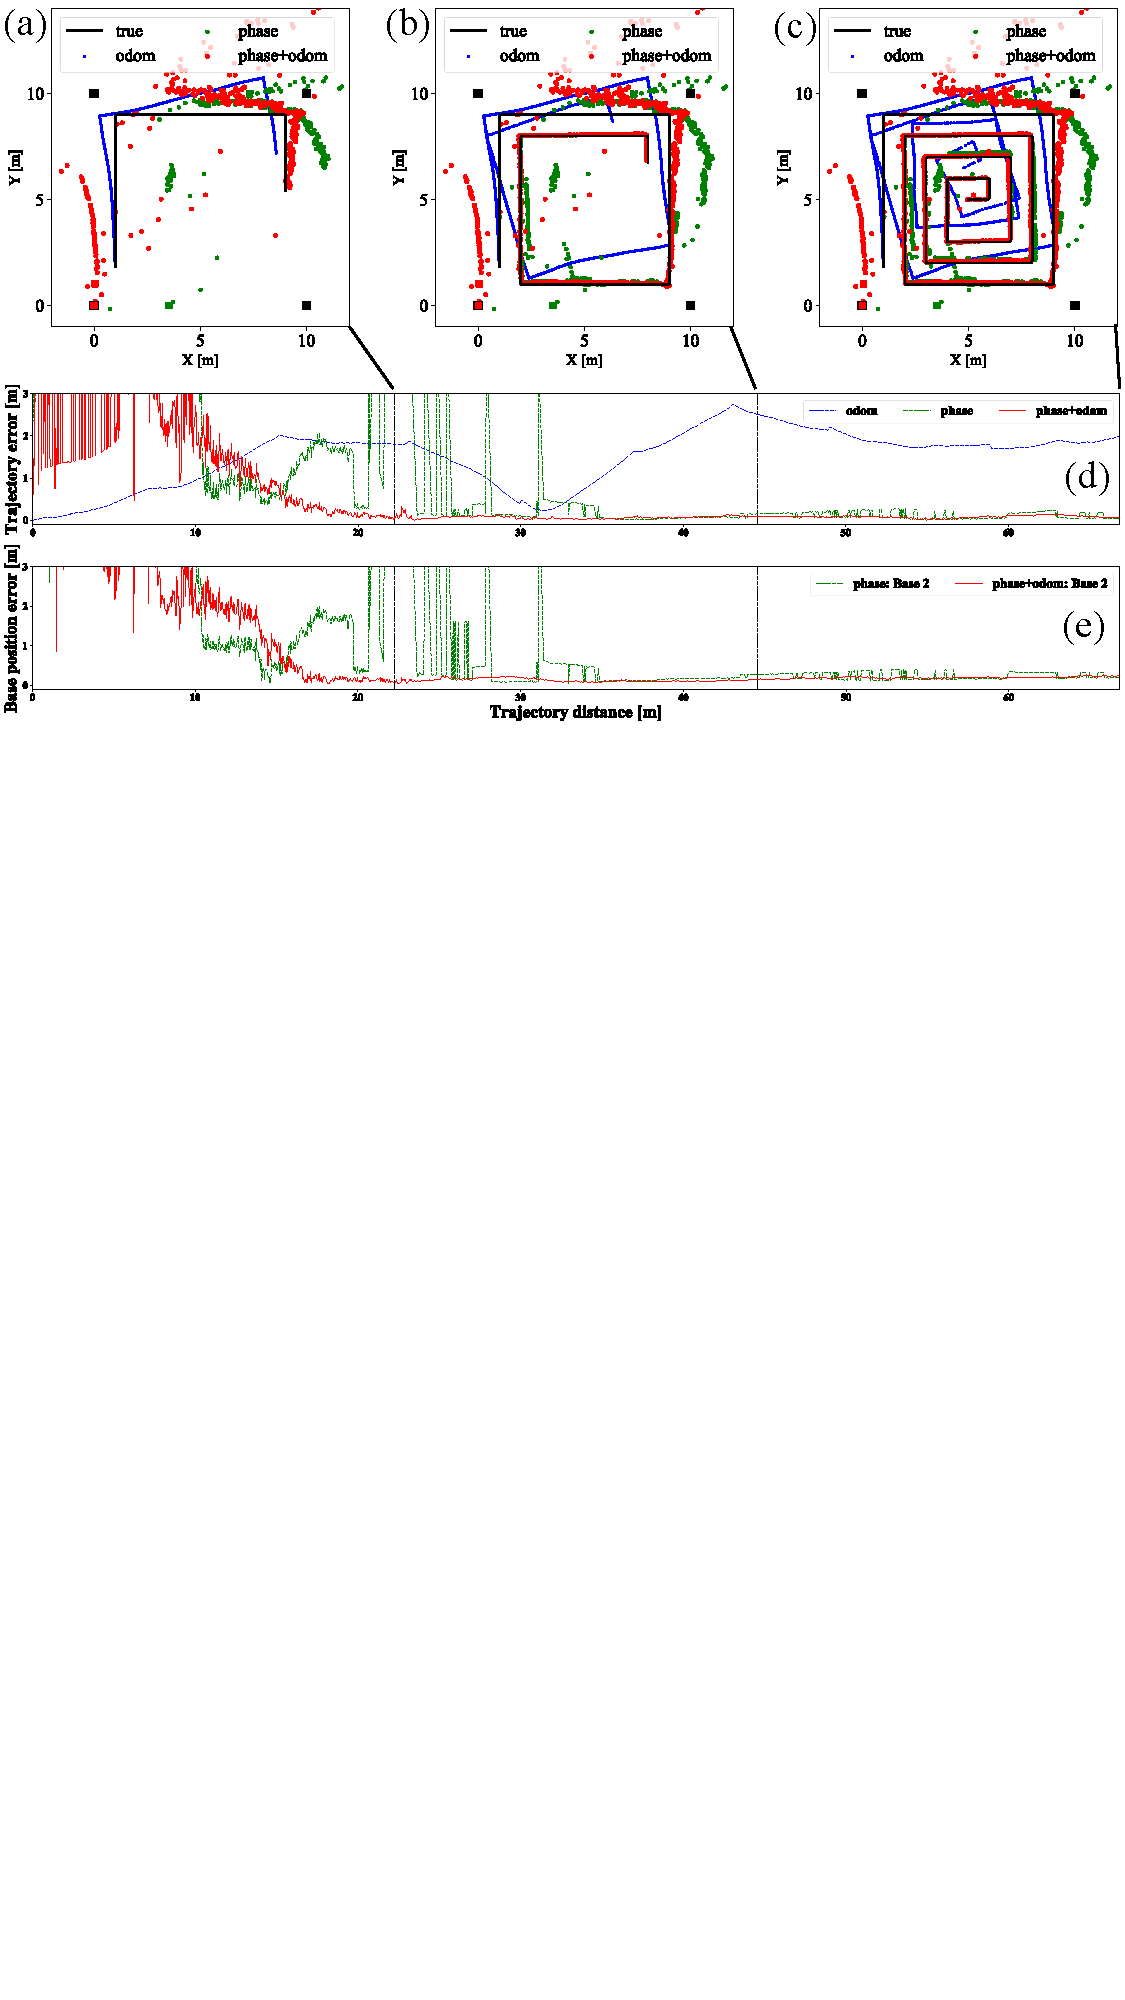
\includegraphics[width=0.95\linewidth]{figures/sim_graph.pdf}
    \caption{Estimation results of robot trajectory and fixed bases position(a,b,c). The red circles, representing the estimated values of the proposed method, gradually converge to the true path. (●: start, ×:goal, and ■: fixed bases numbered 0, 1, 2, and 3 counterclockwise starting from the bottom left.) Graphs (d) and (e) show estimation errors for each condition relative to the trajectory distance. }
    \label{fig:trajectory_sim}
\end{figure*}
% \begin{figure}
%     \centering
%     \includegraphics[width=0.95\linewidth]{figures/robosym_online_rover_position_error_comparison.pdf}
%     \caption{Position estimation errors for each condition relative to the robot's travel distance. 
%     The proposed method, shown by the red line, converges around 20m.}
%     \label{fig:error_sim_robot}
% \end{figure}
% \begin{figure}
%     \centering
%     \includegraphics[width=0.95\linewidth]{figures/robosym_online_base_position_error_comparison.pdf}
%     \caption{Position estimation errors for fixed station $\mathbf{B}_2$ under each condition relative to the robot's travel distance.
%     The proposed method converges around 20m.}
%     \label{fig:error_sim_base}
% \end{figure}
\begin{table}
    \centering
    \caption{Initial values used for the estimation of fixed bases.}
    \begin{tabular}{|c|c|c|c|}
    \hline    
        & $\mathbf{B_1}$ & $\mathbf{B_2}$ & $\mathbf{B_3}$ \\
    \hline    
       True value [m] &(10,0)  &(10,10) &(0,10) \\
       Initial value [m] &(9,0)  &(11,11) &(0,11) \\
    \hline
    \end{tabular}
    \label{tab:initial}
\end{table}

\begin{table}
    \centering
    \caption{Position estimation accuracy for each fixed bases.}
    \begin{tabular}{|c|c|c|c|}
    \hline    
    &$\mathbf{B_1}$ & $\mathbf{B_2}$ & $\mathbf{B_3}$ \\
    \hline    
    phase&0.025m  &0.208m &0.214m \\
    phase+odom &0.043m  &0.168m &0.083m \\
    \hline
    \end{tabular}
    \label{tab:base_error}
\end{table}
以上より,提案手法では,オドメトリの累積誤差を位相計測値で補正しつつ,オドメトリを用いて固定局及びロボットの位置の推定を素早く収束させ,安定して推定を行っていることが確認できた.
\subsection{考察}
シミュレーション実験では,提案手法を用いて固定局の正確な位置関係が未知の状態から固定局の位置とロボットの軌跡をオンラインで推定できることが分かった.
提案手法では,逐次的に新たな計測データが追加されノード及びエッジの数が増加していく.
そのため,推定結果が収束するまで計測データの収集が必要となる.
一方で,ノードやエッジの数が増加しすぎると,推定に必要な時間も増加するおそれがあり,オンライン推定においては,一定の時間以内に推定を完了させる必要がある.
今後,推定を一定時間内に抑えるリサンプリング手法などの工夫が必要になると考えられる.

%%%%%%%%%%%%%%%%%%%%%%%%%%%%%%%%%%%%%%%%%%%
\section{屋内環境での実機実験評価}
提案手法はGNSSが利用しにくい屋内環境での利用が想定される.
そのため,屋内環境において実機システムを用いた精度検証実験を実施した.
実験に用いた環境は,横7.4m,縦11.2mサイズの居室の一部を用いた.
研究室の居室として利用しているため,机や棚と言った什器が壁面に配置されている.
\subsection{実験システム}
% \figref{system}に実験システムの構成図を示す.
シミュレーション同様,実験システムはROS 1(Noetic)上に実装されている.
Wi-Wi端末は,すべての端末間の位相計測の情報を1つの端末からUSB-Serial経由で取得できる.
固定局の一つを実験用のPCに接続し位相情報を記録する.
ロボットの制御はWi-Fi経由で行い,オドメトリ計測値も実験用PCで記録する.
ロボットの位置や固定局の真値は,モーションキャプチャを用いて120Hzで実験用PCに記録する.

\figref{robot}に実験で使用したロボットと固定局の外観を示す.
ロボットはWi-Wiを用いた搬送波位相計測用に開発したロボットを用いる.
ロボットはメカナム移動台車をベースとし,高さ方向1.3mの位置に送受信アンテナが搭載されている.
ロボットの操作は手動で行いWi-Fi経由で司令値を実験用PCからロボット内の制御PCに送信する.
オドメトリはタイヤの回転数を基にロボット内の制御PCで算出されWi-Fi経由で実験用PCに送信される.
固定局は,三脚上に固定されており,高さ1.3の位置に送受信アンテナが存在する.

\begin{figure}
    \centering
    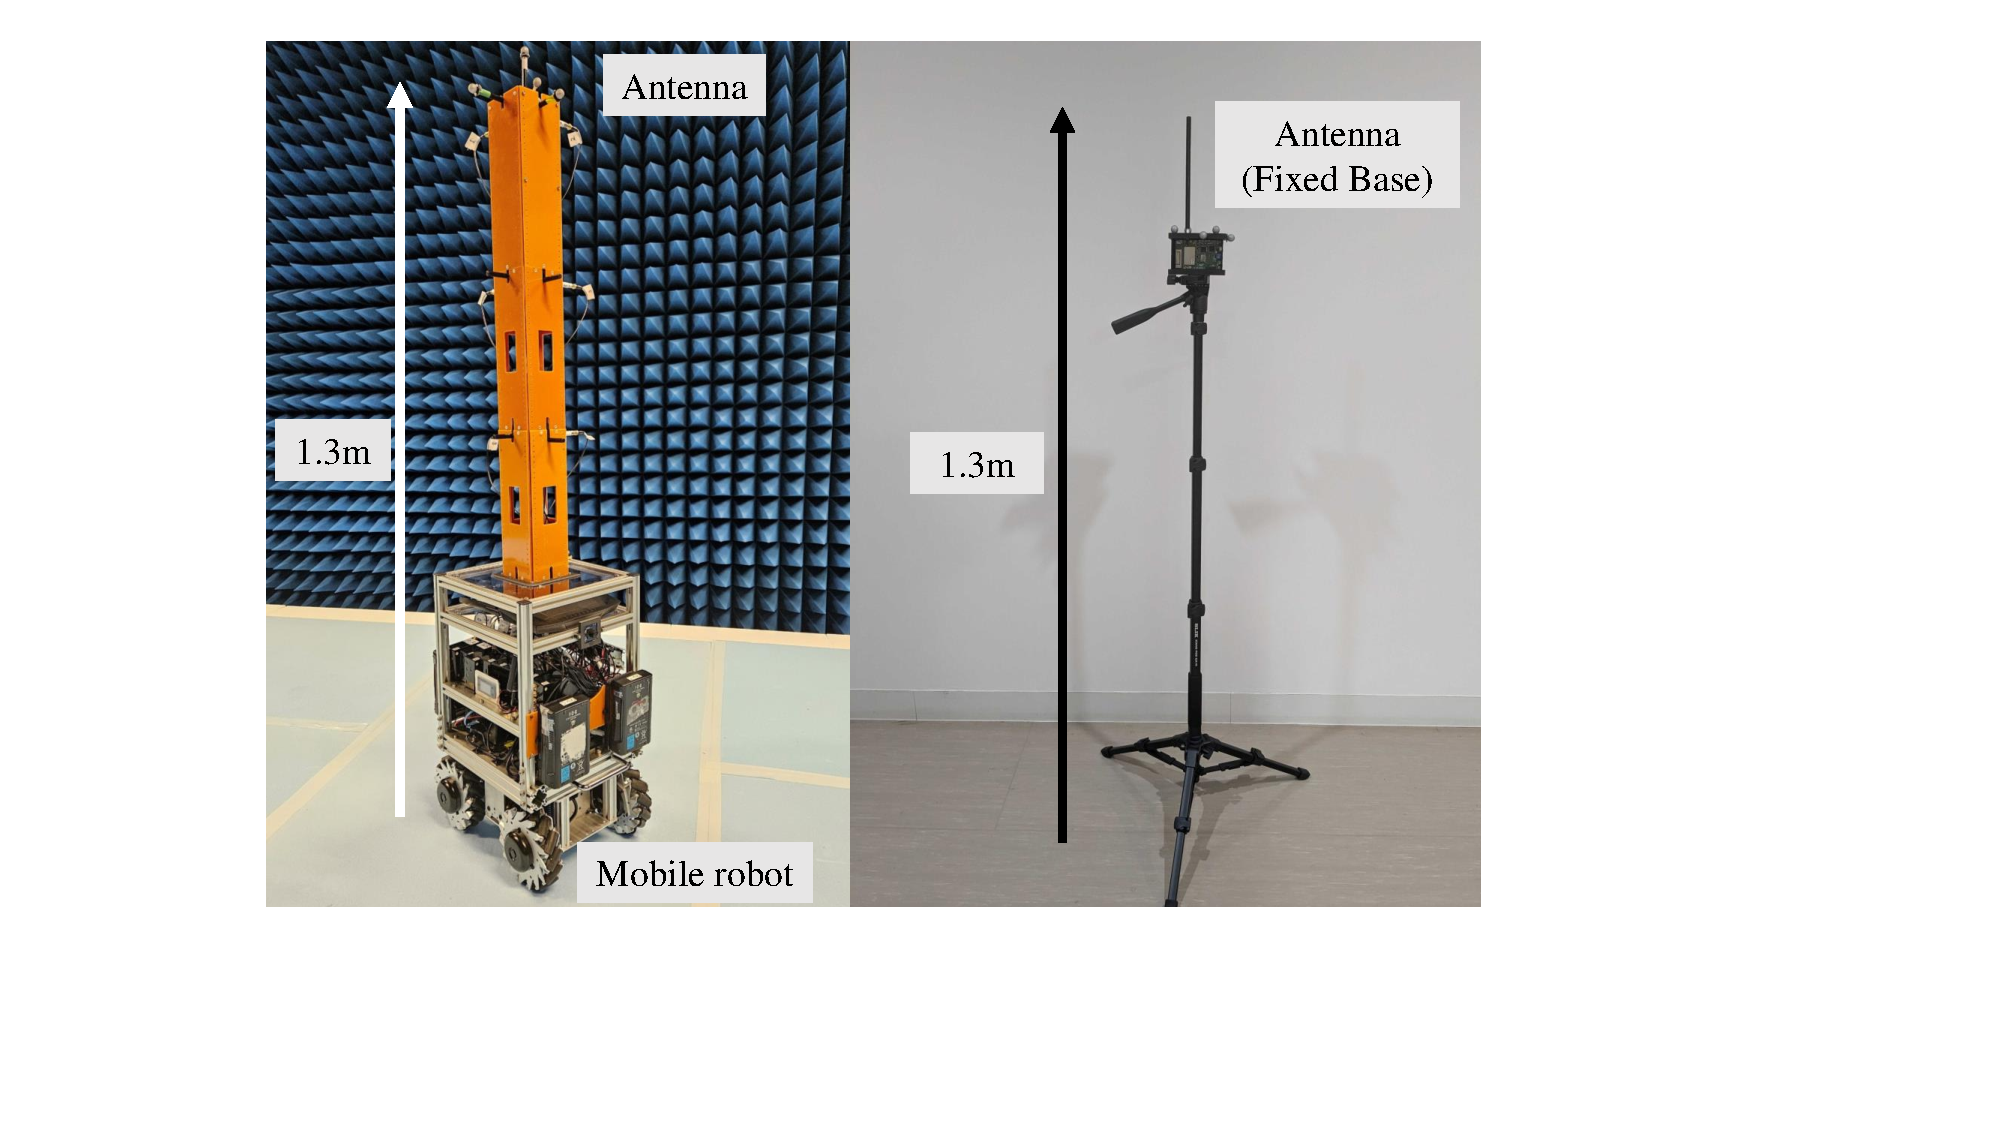
\includegraphics[width=0.95\linewidth]{figures/robot}
    \caption{Appearance of the robot and fixed base used in the experiment}
    \label{fig:robot}
\end{figure}
% \begin{figure}
%     \centering
%     \includegraphics[width=0.95\linewidth]{figures/system.pdf}
%     \caption{実験システムの構成図}
%     \label{fig:system}
% \end{figure}
\subsection{実験条件}
シミュレーションと同様に2次元平面内でのロボットと4台の固定局の位置推定を行う.
固定局の位置と最適化に用いる初期値を\tabref{initial_real}に示す.

ロボットは手動操縦にて環境中を任意に走行させた.
走行距離は約120m,走行時間は約400秒である.
なお実験結果は新たな計測値が追加されるたびに最適化が実行されるオンライン推定方式を取っているが,推定時間がWi-Wiの計測周期である20Hz以内に収まっていないため,現状では,リアルタイム性はない.
\begin{table}
    \centering
    \caption{Initial values used to estimate fixed bases in the experiment.}
    \begin{tabular}{|c|c|c|c|}
    \hline    
        & $\mathbf{B_1}$ & $\mathbf{B_2}$ & $\mathbf{B_3}$ \\
    \hline    
       True value [m]  &(2.79,0)  &(3.58,3.67) &(-0.09,3.67) \\
       Initial value [m] &(3.79,0)  &(3.58,4.67) &(0.91,4.67) \\
    \hline
    \end{tabular}
    \label{tab:initial_real}
\end{table}
\subsection{実験結果}
\figref{error_real}にモーションキャプチャで計測した位置を用いて計算した提案手法の推定誤差を示す.
オドメトリの計測誤差が移動距離に伴い累積していくのに対して,提案手法ではおよそ1m以下の誤差に収まっていることが確認できる.

\tabref{base_error}に経路の終端において推定された固定局の値を示す.
固定局1に関しては0.11mの精度で位置を推定できているが,固定局2では約1.7m,固定局3では0.787mの推定誤差だった.
最も推定誤差の小さかった固定局1と最も誤差の大きかった固定局2の推定誤差の推移を\figref{error_base}に示す.
固定局2では,推定誤差が1.7mあたりに収束してしまっていることが確認できる.

% \begin{figure}
%     \centering
%     \includegraphics[width=0.95\linewidth]{figures/robosym_rover_trajectories_real.pdf}
    
%     \caption{ロボットの移動軌跡(真値,オドメトリのみ,提案手法)}
%     \label{fig:trajectory_real}
% \end{figure}
\begin{figure}
    \centering
    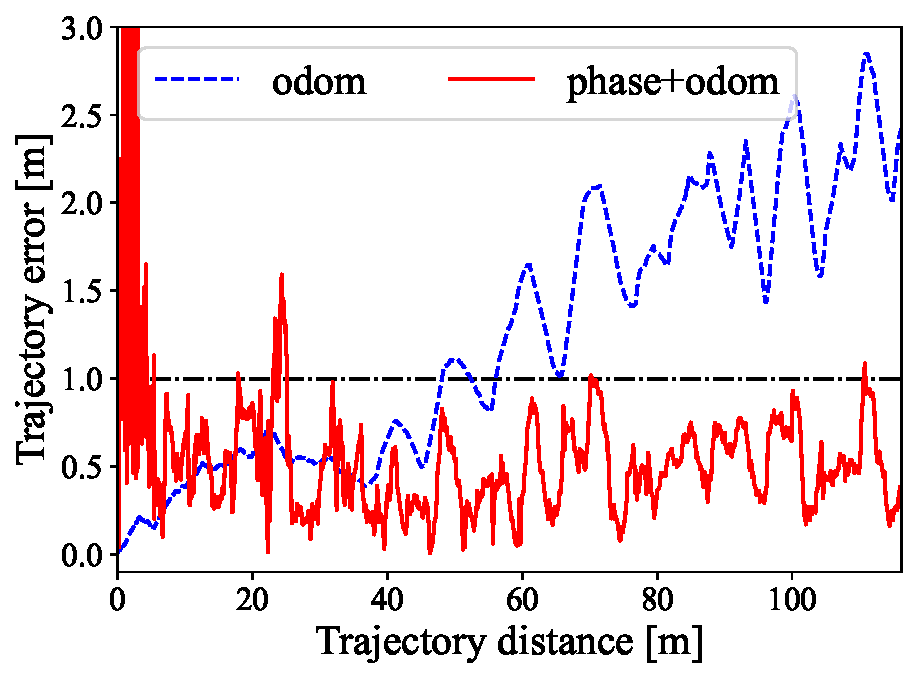
\includegraphics[width=0.95\linewidth]{figures/robosym_online_rover_position_error.pdf}
    \caption{Position estimation errors of the robot relative to the trajectory distance.}
    \label{fig:error_real}
\end{figure}
\begin{figure}
    \centering
    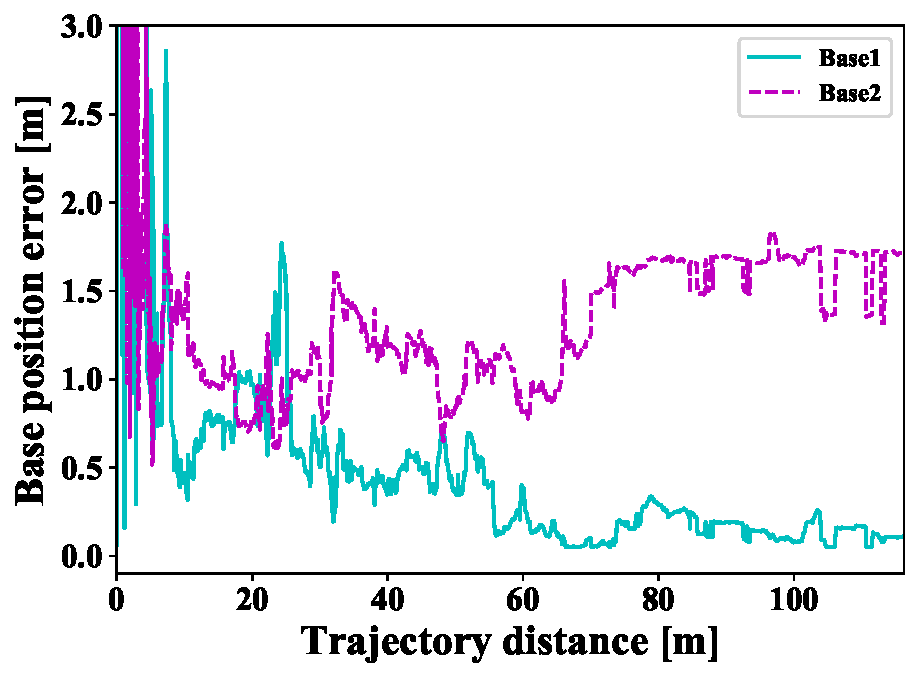
\includegraphics[width=0.95\linewidth]{figures/robosym_online_base_position_error.pdf}
    \caption{Position estimation errors of the bases relative to the trajectory distance.}
    \label{fig:error_base}
\end{figure}
\begin{table}
    \centering
    \caption{Position estimation accuracy for each fixed bases.}
    \begin{tabular}{|c|c|c|c|}
    \hline    
    &$\mathbf{B_1}$ & $\mathbf{B_2}$ & $\mathbf{B_3}$ \\
    \hline    
    phase+odom&0.11m  &1.711m &0.787m \\
    \hline
    \end{tabular}
    \label{tab:base_error}
\end{table}

以上より,提案手法を用いて,GNSSが利用できない屋内環境にユーザーが無線固定局を配置するだけで,移動ロボットの位置を1m以下の精度で推定し,固定局では最小で0.11mの精度で位置が推定できた.

\subsection{考察}
Wi-Wiによる搬送波位相の計測精度の観点から,提案手法の特性,推定精度を考察する.
\figref{vicon_vs_wiwi}に最も誤差が小さかった固定局1に関してモーションキャプチャの計測値から計算した位相差分の参照値と,Wi-Wiからの計測値を元に計算した位相差分の計測値の差分を示す.
ただし,差分の傾向としては4台とも同じ傾向であった.
また,\tabref{vicon_vs_wiwi}に参照値と実測値のRMSE(Root Mean Squared Error)を示す.
Wi-Wiによる搬送波位相差分の平均値は各固定局とも約0.03mの精度で計測できている.
一方\figref{vicon_vs_wiwi}から,スパイク状に計測誤差が増加している箇所が確認できる.
これは,周囲の物体などに反射した反射波の影響が考えられる.
このようなスパイク状の誤差は,すべての固定局で見られたが,最適化を用いて0.1mの精度で位置を推定できているケースが確認された.
一方,1.7m程度の誤差が生じてしまった要因とも考えられる.
今後,反射波の影響を受けた計測値を推定ノードから除外する機能を追加することで,さらなる推定精度の向上が期待される.
\begin{figure}
    \centering
    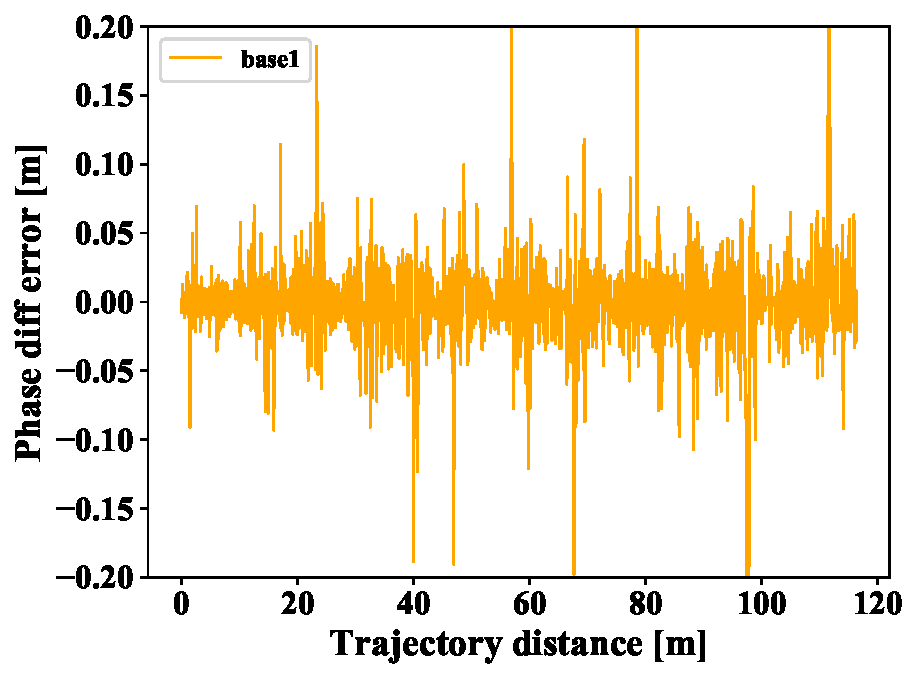
\includegraphics[width=0.99\linewidth]{figures/robosym_distance_pdm_differences.pdf}
    \caption{Difference between the reference phase differences calculated from motion capture and the phase differences measured by Wi-Wi (for base1).}
    \label{fig:vicon_vs_wiwi}
\end{figure}

\begin{table}[tb]
    \centering
    \caption{RMSE between the reference and measured values of phase differences.}
    \begin{tabular}{|c|c|c|c|c|}
    \hline
         &$\mathrm{Base}_0$  &$\mathrm{Base}_1$  &$\mathrm{Base}_2$  &$\mathrm{Base}_3$ \\\hline
     RMSE[m] & 0.035 & 0.027 & 0.029 & 0.025 \\
     \hline
    \end{tabular}
    \label{tab:vicon_vs_wiwi}
\end{table}

\section{結言}
本稿では,搬送波位相とオドメトリを組合せたグラフ最適化用いて,移動ロボットの軌跡と固定局の位置を同時に推定する手法を提案した.
提案手法を実装したシミュレーション実験によって,オドメトリ計測間での搬送波の位相差分を用いることで,オドメトリの累積誤差を修正し,推定精度が向上することを確認した.
実機実験では,電波による位置推定が難しい屋内環境において,固定局の正確な位置関係とロボットの位置が未知の状態から,移動ロボットの位置を1m以下の精度で推定し,固定局では最小で0.11mの精度で位置を推定することができた.
一方で,屋内環境で多く発生する反射波等の影響を完全に抑制できているとはいえず,計測値のフィルタリングの追加やリアルタイム推定に向けた推定時間の短縮などが今後の課題となる.

\begin{acknowledgements}
本研究は,福島国際研究教育機構(F-REI)の委託研究費 (JPFR23010101) により実施した.
\end{acknowledgements}
%---------------------------------------------------------------------
% 参考文献
%--------------------------------------------------------------------
\bibliographystyle{junsrt}
\bibliography{references}
\end{document}
